\documentclass{article}
\usepackage[utf8]{inputenc}
\usepackage[T1]{fontenc}
\usepackage{geometry}
\geometry{a4paper}
\usepackage[english]{babel}
\usepackage{array}
\usepackage{graphicx}
\usepackage{longtable}
\title{Progetto per Basi di Dati}
\author{Mutua Fadhla Mohamed}
\begin{document}
\maketitle
\tableofcontents
\section{Descrizione}
This database contains information on tolls a player needs to pay to be able to travel from one dimension to another (which is unlocked by  completing a set of quests). It needs the player to have a certain amount of achivements completed, be in a guild that is not considered evil (e.g. player killers), have unmodified/achivement complying weapons. All of which is verified by an npc, and only sells them a pass if they checks are TRUE.
\section{Schema concettuale}

\begin{figure}[h!]
    \centering
    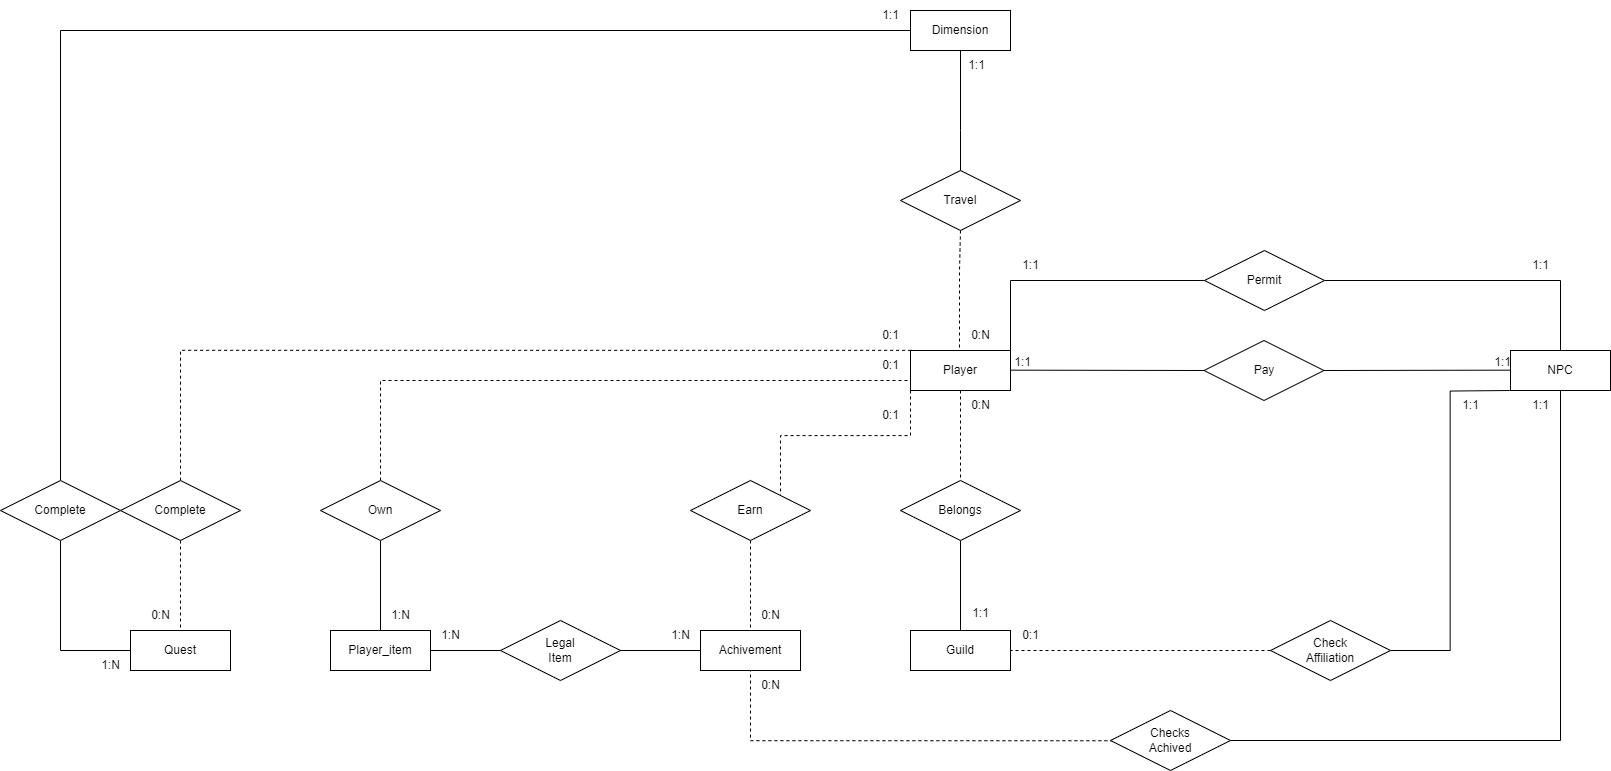
\includegraphics[width=1.2\textwidth]{schema_concetuale.png} % Relative path to your image file
    \caption{Schema concettuale (1)}
    \label{fig:Schema Concettuale}
\end{figure}

% Table E-R
\begin{table}[h!]
    \centering
    \begin{tabular}{ | l | l | l | }
        \hline
        \textbf{Entity 1} & \textbf{Relationship} & \textbf{Entity 2} \\
        \hline
        Player (1:1) & Pay & NPC (1:1) \\
        \hline
        Player (0:1) & Complete & Quest (0:N) \\
        \hline
        Player (0:1) & Own & Player\_item (1:N) \\
        \hline
         Player\_item (1:N) & Legal\_item & Achievement (1:N) \\
        \hline
        Player (0:N) & Belong & Guild (1:1) \\
        \hline
        NPC (1:1) & Checks\_Affiliation & Guild (0:1) \\
        \hline
        NPC (1:1) & Checks\_Achieved & Achievement (0:N) \\
        \hline
        Player (0:N) & Travel & Dimension (1:1) \\
        \hline
        NPC (1:1) & Travel\_permit & Player (1:1) \\
        \hline
        Dimension (1:1) & Complete & Quest(1:N) \\
        \hline
    \end{tabular}
    \caption{Entity-Relationship Descriptions}
    \label{tab:er_descriptions}
\end{table}

\section{Schema Logico}

% Table Entità

\subsection{Entità}


\begin{longtable}{ | l | p{6cm} | p{6cm} | l | l | }
    \hline
    \textbf{Entità} & \textbf{Descrizione} & \textbf{Attributi} & \textbf{Identificato / Primary Key} & \textbf{Foreign Key} \\
    \hline
    Player & A user of the game & player\_id, name, level, experience, guild\_id (nullable) & player\_id & guild\_id \\
    \hline
    NPC & Non-player character & npc\_id, name, role, alignment & npc\_id & \\
    \hline
    Quest & A task or mission & quest\_id, name, description, reward & quest\_id & \\
    \hline
    Player\_Item & Items owned by a player & player\_item\_id, player\_id, item\_id, quantity & player\_item\_id & player\_id, item\_id \\
    \hline
    Item & Items in the game & item\_id, name, type, value & item\_id & \\
    \hline
    Achievement & Achievements earned by players & achievement\_id, name, description & achievement\_id & \\
    \hline
    Guild & Groups that players can join & guild\_id, name, alignment & guild\_id & \\
    \hline
    Dimension & Different game worlds or levels & dimension\_id, name, description & dimension\_id & \\
    \hline
    Payment & Payments made by players to NPCs & payment\_id, player\_id, npc\_id, amount, timestamp & payment\_id & player\_id, npc\_id \\
    \hline
    Completion & Record of completed quests & completion\_id, player\_id, quest\_id, completion\_date & completion\_id & player\_id, quest\_id \\
    \hline
    Earn & Record of earned achievements & earn\_id, player\_id, achievement\_id, earn\_date & earn\_id & player\_id, achievement\_id \\
    \hline
    Travel & Records of player travels & travel\_id, player\_id, dimension\_id, permit (Boolean) & travel\_id & player\_id, dimension\_id \\
    \hline
\end{longtable}

% Table Relazioni

\subsection{Relazioni}

\begin{center}
 \begin{small}
\begin{longtable}{ | l | p{6cm} | p{6cm} | p{6cm} | l | l | }
    \hline
    \textbf{Relazioni} & \textbf{Descrizione} & \textbf{Componenti} & \textbf{Attributi} & \textbf{Identificato / Primary Key} & \textbf{Foreign Key} \\
    \hline
    Pay & Payment from player to NPC & Player (1:1), NPC (1:1) & payment\_id, player\_id, npc\_id, amount, timestamp & payment\_id & player\_id, npc\_id \\
    \hline
    Complete & Completion of quests by players & Player (0:1), Quest (0:N) & completion\_id, player\_id, quest\_id, completion\_date & completion\_id & player\_id, quest\_id \\
    \hline
    Own & Ownership of items by players & Player (0:1), Player\_Item (1:N) & player\_item\_id, player\_id, item\_id, quantity & player\_item\_id & player\_id, item\_id \\
    \hline
    Earn & Earning of achievements by players & Player (0:1), Achievement (0:N) & earn\_id, player\_id, achievement\_id, earn\_date & earn\_id & player\_id, achievement\_id \\
    \hline
    Belong & Membership of players in guilds & Player (0:1), Guild (1:N) & guild\_id & player\_id & guild\_id \\
    \hline
    Checks\_Alignment & NPC checks alignment of guild & NPC (1:1), Guild (0:1) & npc\_id, guild\_id & & npc\_id, guild\_id \\
    \hline
    Checks\_Achievement & NPC checks player's achievements & NPC (1:1), Achievement (0:N) & npc\_id, achievement\_id & & npc\_id, achievement\_id \\
    \hline
    Checks\_Illegal\_items & NPC checks player's items & NPC (1:1), Player\_Item (0:N) & npc\_id, player\_item\_id & & npc\_id, player\_item\_id \\
    \hline
    Checks\_Quest & NPC checks player's quests & NPC (1:1), Quest (0:N) & npc\_id, quest\_id & & npc\_id, quest\_id \\
    \hline
    Travel & Player travels to a dimension & Player (0:N), Dimension (1:1) & travel\_id, player\_id, dimension\_id, permit (Boolean) & travel\_id & player\_id, dimension\_id \\
    \hline
    Travel\_permit & NPC grants travel permits to dimensions & NPC (1:1), Dimension (1:1) & npc\_id, dimension\_id & & npc\_id, dimension\_id \\
    \hline
\end{longtable}
\end{small}
\end{center}

\end{document}